\documentclass[12pt,english]{article}
%\usepackage{lmodern}
\linespread{1.05}
\usepackage{mathpazo}
%\usepackage{mathptmx}
%\usepackage{utopia}
\usepackage{microtype}
\usepackage[T1]{fontenc}
\usepackage[latin9]{inputenc}
\usepackage[dvipsnames]{xcolor}
\usepackage{geometry}
\usepackage{amsthm}
\usepackage{amsfonts}

\usepackage{courier}
\usepackage{verbatim}
\usepackage[round]{natbib}
\bibliographystyle{plainnat}


\definecolor{red1}{RGB}{128,0,0}
%\geometry{verbose,tmargin=1.25in,bmargin=1.25in,lmargin=1.25in,rmargin=1.25in}
\geometry{verbose,tmargin=1in,bmargin=1in,lmargin=1in,rmargin=1in}
\usepackage{setspace}

\usepackage[colorlinks=true, linkcolor={red!70!black}, citecolor={blue!50!black}, urlcolor={blue!80!black}]{hyperref}
%\usepackage{esint}
\onehalfspacing
\usepackage{babel}
\usepackage{amsmath}
\usepackage{graphicx}

\theoremstyle{remark}
\newtheorem{remark}{Remark}
\begin{document}
	
\title{Endogenous Growth with Creative Destruction by Employee Spinouts}
\author{Nicolas Fernandez-Arias}
\maketitle

\textbf{Moll: get to point faster.} \newline
\textbf{Ezra: reduce emphasis on comparing to similar work. just say what you did. also, be gentle when discussing other work.}

\section{Introduction}
Silicon Valley (SV) is often hailed as a paragon of economic dynamism and innovation. And not without reason: labor productivity growth in the MSA containing SV averaged 2.72\% from 1978 to 2015, compared to an average of about 2\% for the whole country. This difference in growth rates implies a 30\% increase in the level of productivity over the time period, which likely underestimates the contribution to aggregate labor productivity growth for several reasons. \footnote{See \cite{parilla_understanding_2017}. Further, the employment growth rate exceeded the national average during this time period, increasing the contribution to aggregate labor productivity growth. Even more importantly, labor productivity growth in SV has been centered on ICT-producing firms, whose output contributes heavily to labor productivity growth in other industries. \cite{jorgenson_retrospective_2008} attributes nearly half of labor productivity growth from 1973-2006 (and more 60\% from 1995-2000) to ICT. Consistent with this, the appendix of  \cite{parilla_understanding_2017} reports that labor productivity growth peaked at almost 5\% annualized in the MSA containing SV from the years 1994-2005.} The literature has argued for the importance of employee mobility and entrepreneurship in the region, with a particularly important part played by \textit{employee spinouts}: firms founded by former employees in the same or related industries as the former employer. \footnote{See \cite{saxenian_regional_1994}, \cite{gilson_legal_1999}, \cite{fallick_job-hopping_2006}, \cite{franco_covenants_2008}.} \footnote{This is different from a "spinoff", which is a division of a firm that the firm itself decides to sell. The early literature uses these terms interchangeably, but the more recent literature has settled on the term "spinout" for entrepreneurship initiated by the employee.} As an anecdotal illustration, Figure \ref{fairchild_spinouts} shows the many direct and indirect spinouts of Fairchild Semiconductor, one of the first leading semiconductor firms of SV -- itself a spinout of Shockley Laboratories, another semiconductor firm. Although Fairchild was founded in the 1950s, its list of spinouts includes some of the most well-known modern firms in SV, such as Intel and AMD. In turn, the literature has hypothesized that SV's unusual rates of employee mobility and entrepreneurship are due to California's prohibition on the enforcement of covenants not to compete (CNCs). \footnote{\cite{saxenian_regional_1994} attributes SV's rise from the 1960s to the 1990s (relative to Route 128 in Massachusetts, the previous tech hub) to SV's higher degree of employee mobility and entrepreneurship, as well as to its modular industrial structure. In turn, \cite{gilson_legal_1999} argues that this resulted from California's state-level statue not to enforce a labor contract known as a covenant not to compete (CNC), or simply non-compete.  \cite{fallick_job-hopping_2006} complements this view using survey data from the CPS, providing evidence that employee mobility is (1) higher in the computer industry in SV than in computer industries in other regions, and (2) higher in the computer industry in California than in the computer industries outside of California. The authors interpret this as evidence of a California-level factor rather than something SV-specific, and suggest an interpretation in line with the hypothesis of \cite{gilson_legal_1999}. Finally, \cite{franco_covenants_2008} considers a two-region model of spinout formation with and without CNCs in which the enforcing region has more initial firm entry but is eventually overtaken by the non-enforcing region.} Such contracts prevent departing employees from joining or founding competing firms for a span of time (usually 6 months to 2 years) and often in a certain geographical region. Figure \ref{noncompetes_enforcement} illustrates the state-level cross-sectional variation in the degree of enforceability of such contracts. California's lack of enforcement is far from typical.

\begin{figure}	\phantomsection
	\center
	\includegraphics[scale = 0.77]{../figures/fairchildren_early.png}
	\caption{Direct and indirect spinouts of Fairchild Semiconductor}
	\label{fairchild_spinouts}
\end{figure}

\begin{figure}	\phantomsection
	\center
	\caption{State-level enforceability of CNCs. Source: Bishara 2011}
	\includegraphics[scale = 0.68]{../figures/noncompetes_enforcement.png}
	\label{noncompetes_enforcement}
\end{figure}



Of course, the specific cause of SV's rise is difficult to ascertain. Nevertheless, the preceding question motivates the general question of what effect spinout entrepreneurship -- and in particular enforceability of non-competes -- has on innovation and labor productivity growth. This paper attempts to take a step towards answering this question.

In order to do so, I employ the following methodology. I develop a model of endogenous growth in which employees learn on the job how to form spinout firms.\footnote{The model is based on the framework in \cite{akcigit_growth_2018}, which follows the seminal work \cite{grossman_quality_1991}. The expanding-variety endogenous growth models based on \cite{romer_increasing_1986} are not suitable for my analysis, where creative destruction is essential.} The model has two versions: one in which workers have commitment (i.e. CNCs can be enforced) and another in which they do not. According to the model, two key parameters determine the productivity growth / welfare comparison between the two regimes: (1) the rate of employee spinout idea discovery, and (2) the degree to which spinout profits come at the expense of the profit of the parent firm. Typically, in the non-enforcement regime, the effect on growth and welfare of increasing the rate of employee learning -- which expands the production possibilities frontier -- is non-monotonic.\footnote{Note that this implies it is inefficient. I am working on solving the social planner's problem using \cite{nuno_social_2018}.} I provide some empirical discipline on these parameters by exploiting a dataset assembled from micro data on VC-funded startups (Venture Source), R\&D information in Compustat/CRSP, NBER and USPTO patent data, and state- and federal-level R\&D subsidies in Bloom et al. 2013. I discipline the other parameters of the model using indirect inference.\footnote{There are two ways to do this: calibrate the no-commitment model with data from California, or calibrate the commitment model with data from states which do enforce.} I validate the model by comparing its predictions to previously documented patterns from the spinout literature (in progress). Finally, I use the model to study the growth effects of policies that discourage or encourage spinout formation, such as non-compete enforcement but also R\&D subsidies for entering firms.

Several strands of the literature point to the importance of answering this question. A large literature that has argued for the importance of business entry in labor productivity growth.\footnote{Using an accounting decomposition, \cite{foster_aggregate_2001} estimates that entry accounts for 25\% of aggregate productivity growth in the United States. See \cite{brandt_creative_2012} for evidence from China. See \cite{asturias_firm_2019} for evidence from Chile and Korea. \cite{akcigit_growth_2018} arrives at a similar estimate using a structural approach disciplined by patent citations data.} Another empirical literature has documented that employee spinouts are more productive, grow faster, and survive longer than other entrants.\footnote{See \cite{baslandze_spinout_2019} for evidence from US patent data and Compustat. See \cite{muendler_employee_2012} for evidence from Brazilian employer-employee matched data.} A related literature has argued that spinouts inherit knowledge from their parents, and that parent firms tend to be productive and knowledge intensive.\footnote{See \cite{klepper_entry_2005}, \cite{gompers_entrepreneurial_2005}, and \cite{baslandze_spinout_2019}.} 

\textbf{[need to more clearly distinguish between competing spinouts and non-competing spinouts. this part needs to be reworked.]}
Theory suggests that the answer to this question is non-trivial. As pointed out by Schumpter, \cite{arrow_economic_1962}, and more recently \cite{romer_increasing_1986}, the limited excludability of knowledge means the returns to investment cannot be fully appropriated. If CNC enforcement reduces the formation of spinouts, incumbent firms can better appropriate the returns of knowledge (or capital) investments. By increasing appropriability, CNC enforcement induces more investment by incumbent firms in equilibrium. CNCs play a role similar to patents, which also incentivize investment in knowledge by reducing knowledge spillovers and competition.

However, note that in the case of employee spinouts, the employee can only appropriate the firm's investments because of his contractual relationship with the employer  (i.e., because he working for her).  Therefore, as highlighted by \cite{franco_spin-outs:_2006}, incumbent firms will be compensated for this lost value in the form of lower equilibrium wages. This occurs due to employees pricing in the value of the know-how they acquire on the job. In that model, even without CNC enforcement, the equilibrium is Pareto efficient. A crucial assumption, though, is that spinouts do not compete directly with the parent firm. If they do, the potential to form a spinout reduces the bilateral value of the firm and employee. The effective wage paid by the firm -- taking into account the potential lost value from competition -- is higher than if there were a CNC. This reduces the incentive to invest in knowledge. 

On the other hand, even if CNCs allow incumbent firms and their employees to write a bilaterally more efficient contract, incumbents will in general still underinvest in R\&D relative to the social optimum due to monopoly power. Forcing them to allow spinouts may increase efficiency by increasing knowledge diffusion and producing firms motivated by creative destruction. Such firms invest a socially excessive amount in R\&D due to business-stealing, which may offset the underinvestment by incumbent firms.\footnote{This is one of the insights from the literature spawned by \cite{grossman_quality_1991}. In the basic models, the effect of business stealing on equilibrium innovation rates is stark: incumbent firms are entirely priced out of innovation by firms attempting creative destruction.}

Finally, politically, there is a significant amount of momentum towards limiting the enforcement of CNCs, both at the federal and state level. In 2015 Hawaii banned non-competes for technology workers. In 2018, Massachusetts passed legislation significantly limiting the scope of enforceable CNCs. Other states have recently made similar proposals.\footnote{See \cite{the_white_house_technical_report_non-compete_2016}.} In light of this, there is an urgent need to improve our understanding of the issue. 

\paragraph{Related literature}

Some work has attempted to answer this question directly using empirical methods. Papers in this literature have typically used either cross-sectional and/or longitudinal variation in the state-level enforcement of non-competes.\footnote{Sometimes this variation is argued to be exogenous, either due to legislative error as in \cite{marx_mobility_2009} and \cite{marx_regional_2015}, or due to unexpected judicial precedent as in \cite{jeffers_impact_2018}. Often there is a control industry that is believed to be unaffected by the variation in CNC enforcement policy (e.g. law firms are typically exempt from CNC restrictions).} The results are inconclusive and suggest an important tradeoff between entry of spinouts and investment by incumbent firms. \cite{stuart_liquidity_2003} find more local  entrepreneurship in response to local IPO (a "liquidity event") in regions not enforcing CNCs. \cite{marx_mobility_2009} finds that inventor mobility declines in response to an increase in non-compete enforcement. \cite{samila_venture_2010} finds that an increase in VC funding supply increases entrepreneurship more in states without non-compete restrictions, using an IV design. \cite{garmaise_ties_2011} finds that, in states where CNCs are more enforceable, managers are less mobile, have lower compensation, and invest less in their human capital, to the point of offsetting increased investments by the firm. On the other hand, \cite{conti_non-competition_2014} finds evidence that non-compete enforceability leads to incumbent firms pursuing riskier R\&D projects. \cite{colombo_does_2013} finds evidence that easier spinout formation -- proxied by access to finance -- leads to a reduction in incumbent firm knowledge investments.  Most recently, \cite{jeffers_impact_2018} uses data on influential state-level court precedents matched with LinkedIn data and finds that enforcement indeed reduces spinout formation while increasing capital investment by incumbent firms. Finally, \cite{marx_regional_2015} finds that CNC enforcement leads to inventor mobility out of the state, suggesting that differences in outcomes could be in part due to reallocation. 

Theoretical work has also explored this question. As mentioned previously, \cite{franco_spin-outs:_2006} develops a model in which employees learn from their employers and use this knowledge to form spinouts. They emphasizes the "paying for knowledge" effect, whereby employees implicitly pay for the knowledge they take from the parent firm through lower equilibrium wages. Importantly, they assume spinout firms do not steal business from their parents: the only effect of a spinout on the parent firm is a reduction in the price of the output good, which the parent firm is assumed not to take into account. This, combined with the "paying for knowledge" mechanism, ensures that the competitive equilibrium allocation is Pareto efficient, even without resorting to elaborate labor contracts.

\cite{franco_covenants_2008} studies a two-period, two-region model with employee spinouts in which the region which does not enforce CNCs initially lags but eventually overtakes the region in which CNCs are enforced. In the first period, entry is more valuable in the enforcing region. But in the second period, spinouts enter in the non-enforcing region, there is Cournot competition with parent firms in the product market, and output increases relative to the enforcing region. The analysis emphasizes how asymmetric information about whether an employee has learned leads some firms in the non-enforcing region to allow spinouts (assuming firms cannot commit to wage backloading). This can be taken as a rough microfoundation of my assumption that labor contracts are "simple" in  a non-enforcing region: just a wage, with no attempts at retention in the case of learning. They do not consider long-run growth implications, and use a two period model. Spinouts do not worry about spinouts of their own. R\&D is not present - only entry in the first period leads to a certain chance of spinout formation in the second period. 

\cite{shi_restrictions_2018} uses a rich model of contracting disciplined by data on executive non-compete contracts to study the effect of non-competes on executive mobility and firm investment. She finds that the optimal policy is to somewhat restrict the permitted duration of CNCs. Her approach allows her to study the optimal contracting problem in more detail than in mine. However, she is mainly interested in poaching, which involves an attempt to extract a payout from the poaching firm, while I am interested in spinouts. Also, her calibration relies heavily on matching the response of firm investment to the presence of a CNC in the manager's contract. However, she uses capital investment rather than investment in knowledge. This leads her to estimate an R\&D elasticity such that non-competes do not do much to increase the incentives for firm investment. However, I am interested in long-run growth, which is driven by investments in knowledge (in the data, R\&D not capex).

\cite{baslandze_spinout_2019}, the study closest to this paper, studies the effect of spinout entrepreneurship on entry and growth. Baslandze's analysis concludes that the optimal enforcement of non-competes is zero. However, in her framework, spinouts do not steal business from the parent firm, instead entering into a different product line. The harm to the parent firm results from the additional assumption that the parent firm's technology gap -- relative to potential entrants in its own product-line -- drops to zero upon spinout formation. This is modeled as other firms "catching up" technologically to the incumbent, although it is interpreted as the loss of match-specific productivity. In other words, the knowledge of the firm is fully embodied in its R\&D manager. My paper focuses instead on creative destruction of the parent firm using knowledge that is embodied in the firm but can be used simultaneously by the employee in a spinout.  More importantly, in her analysis, higher non-compete enforcement is modeled as a higher cost of spinout formation. This is unsatisfactory because it precludes the possibility that bilaterally efficient spinouts will be allowed even in CNC enforcing regions. 

In addition, the preceding studies are not disciplined by an empirical measurement of the extent to which spinout firms reduce bilateral value, as opposed to simply entering other markets using similar technology. Given the theoretical analysis above, this is critical to the question of whether the decentralized equilibrium is efficient, either with or without elaborate labor contracts. The contribution of this paper is to provide some empirical measurement on this quantity, along with a framework that models its effect on the key outcomes of interest: labor productivity growth and -- taking into account the cost of investment -- the present discounted value of output per person (welfare in my model).

The structure of this paper is the following. In Section \ref{related_literature}, I review some of the related literature. In Section \ref{simplified_model}, I describe a simplified version of the model which is easier to analyze. Section \ref{full_model} describes the full model which will be used in the quantitative analysis. In Section \ref{empirics}, I describe my plan for the empirical strategy. In Section \ref{quantitative_analysis}, I conduct a preliminary calibration exercise, describe the equilibrium, and perform some comparative statics. I show that the effect on the output growth and the present value of consumption of increasing the rate of spinout formation is non-monotonic. Because this is an expansion of the production possibilities frontier, this implies that the equilibrium is inefficient. In the current (preliminary) calibration, the marginal effect of increasing the rate of spinout formation is positive. 

\section{Related literature (bring into intro)}\label{related_literature}

(in progress)

This paper relates to several existing branches of the literature. 

First, there is a long empirical literature on the innovative activities of firms; see \cite{cohen_fifty_2010} for an excellent survey.

Literature on spinoffs and knowledge appropration: \cite{anton_expropriation_1994}, \cite{anton_start-ups_1995}, \cite{franco_covenants_2008}, \cite{klepper_entry_2005}, \cite{klette_innovating_2004}, \cite{chatterjee_spinoffs_2012}

Literature on endogenous growth: \cite{grossman_quality_1991}, \cite{romer_increasing_1986}, \cite{aghion_model_1992}

Literature on non-competes: \cite{saxenian_regional_1994}, \cite{gilson_legal_1999}, \cite{jeffers_impact_2018}, \cite{marx_mobility_2009}, \cite{marx_regional_2015}, \cite{starr_noncompetes_2019}

Literature on the relationship between competition and innovation: \cite{aghion_competition_2005}

\section{Simplified model}\label{simplified_model}

In this section I will describe a simplified version of the full model that illustrates some of the key mechanisms. This version of the model has a simpler equilibrium characterization and statement of the planner problem. The key difference relative to the full model is that the rate of creative destruction by spinouts depends only on the flow of R\&D employment rather than on the stock of past R\&D employment. This eliminates the incentive to increase technological distance from existing potential spinouts, analogous to the \textit{escape competition} effect in \cite{aghion_competition_2005}. As in that model, this effect moderates the disincentive effects of competition.

\subsection{Preferences and Production Technology}

The economy is in continuous time. Households are risk-neutral with discount rate $\rho$. Household $i \in [0,1]$ at time $t$ has objective
\begin{align*}
 \mathbb{E}_t \int_0^{\infty} e^{-\rho s} c(t+s) ds
\end{align*}

Individuals consume a unique final good $Y(t)$, which is produced competitively by labor and a continuum of intermediate goods $j \in [0,1]$ with production technology\footnote{This production function is Cobb-Douglas across labor and a CES aggregator of intermediate goods $j$, weighted by quality. }
\begin{align*}
Y(t) &= \frac{L_F^{\beta}(t)}{1-\beta} \int_0^1 q_j^{\beta}(t) k_j^{1-\beta} (t) dj
\end{align*}

where $k_j(t)$ is the quantity of intermediate good $j$ and $q_j(t)$ is its quality. The price of the final good is normalized to 1 in every period. From now on I will suppress $t$ subscripts when it is clear. 

At any time $t$, to each intermediate good $j$ there corresponds a firm $j$ with a monopoly on its production.\footnote{Although they make decisions independently, like separate firms, it is best to interpret these firms as products. Otherwise the model interprets all entry as new firm entry, rather than some entry being due to creative destruction by existing firms.} Firm $j$ produces its intermediate good with a linear technology
\begin{align*}
k_j = Q l_j
\end{align*}
where $l_j$ is the labor input and $Q = \int_0^1 q_j dj$.

Individuals work in three capacities: final good production ($l_F^i$), intermediate good production ($l_I^i$), and R\&D ($l_{RD}^i$). They also can run firms when they learn how to do so, but they do not need to supply labor to do this. Hence their time constraint is
\begin{align*}
	l_F^i + l_I^i + l_{RD}^i \le 1
\end{align*}

Labor is supplied inelastically (individuals do not value leisure). Letting $L_F = \int_0^1 l_F^i di$ and defining $L_I,L_{RD}$ analogously, the labor market satisfies the resource constraint
\begin{align}
L_F + L_I + L_{RD} &= 1 \label{labor_resource_constraint}
\end{align}

There is no storage technology for consumption, so in equilibrium 
\begin{align*}
Y = C
\end{align*}

\subsection{Research and Development}

The below describes the innovations technologies available to agents in the economy working on a good $j$ with quality $q$ at a time when aggregate TFP is $Q$. As is standard with quality ladders models, R\&D productivity scales with $q$ so that the equilibrium growth rate is independent of $q$.\footnote{This permits solving the model without tracking the evolution of the distribution of $q$ (other than its mean $Q$).}

\subsubsection{Own-innovation by incumbents}

The current producer of good $j$ has a temporary monopoly on the production of good $j$. During this time, he can hire labor to produce the good $j$ or to conduct R\&D to improve the quality of the good (at no increase in costs). Alternatively, the firm can hire $\big(\frac{q}{Q}\big)z_I$ units of R\&D labor in exchange for a Poisson arrival rate of innovations
\begin{align}
\tau_I &= \chi_I z_I \phi(z_I)  \label{incumbent_innovation_rate}
\end{align}
where $\phi(z) = z^{-\psi}$ for exogenous $\psi \in (0,1)$.\footnote{Theoretically, all that is needed is (1) $\phi(z)$ decreasing, (2) $z\phi_I(z)$ increasing, and (3) Inada conditions on $\phi$: $\lim_{z \to 0} \phi'(z) = \infty, \lim_{z \to \infty} \phi'(z) = 0$.}

If the incumbent is the first to receive an innovation arrival, he keeps his monopoly but now produces a good of quality $\lambda q$, where $\lambda > 1$ is an exogenous parameter. 

\subsubsection{Creative destruction}

\paragraph{Entrants} For each $j$, there is a unit mass of entrants owned in equal share by the households who have free entry into R\&D efforts to improve good $j$. As is standard in the quality ladders framework, this means that as soon as an innovation occurs, they can pay cost $Cq_j$ to gain the technology to attempt to innovate on it. If the quality of good $j$ is $q_j$, this technology converts $(\frac{q_j}{Q}) z$ units of flow labor into a Poisson arrival rate of innovations
\begin{align}
	\tau_E &= \chi_E z_E \label{simplified_entrant_innovation_rate}
\end{align}


\paragraph{Spinouts} If a firm -- incumbent or potential entrant -- innovating on good $j$ hires $z$ units of R\&D labor from a worker, with Poisson intensity $\chi_S z$ the worker gains the technology to produce good $j$ at quality $\lambda q_j$ by paying the fixed cost $C q_j$ in terms of the final good.\footnote{There is no opportunity cost labor allocated to managing the firm due to tractability. This cost would inherently scale with the average economy rather than $q_j$, destroying the linear scaling of the firm value. This is a natural economic assumption - low $q/Q$ firms should exit and be replaced by average $q \approx Q$ entrants. And several models of this type have been studied in the literature (e.g. \cite{acemoglu_innovation_2015}, ), typically yielding a Pareto stationary distribution in $q/Q$, given assumptions generated proportional growth and an (endogenous) lower exit threshold. However, this requires tracking the entire $q$ distribution over time in order to aggregate from individual policies. Solving such a model is possible in this case, but it defeats the purpose of this analytical framework. Also, the model would still have to be modified, since as currently written it would not admit a stationary distribution hence there would likely not be a balanced growth path. In the full model discussed later, there is already a state variable, so adding this would yield a problem with two unbounded continuous state variables, which while potentially feasible may be a signficant challenge to solve numerically.} In equilibrium, provided $C$ is low enough, the R\&D worker does this. This leads to
\begin{align}
	\tau_S &= \chi_S z_I \label{simplified_spinout_innovation_rate}
\end{align}

In the case of a spinout, the worker continues to supply his labor on the labor market. In other words, there is no opportunity cost of forming a spinout from foregone labor earnings. Hence he always forms a spinout. The result is that at a constant rate $\chi_S$ per unit of R\&D effort, an R\&D worker is able to form a spinout, and does so. The model can also be interpreted as the worker selling the spinout for its full value to a competitive fringe of investors owned in equal shares by the household sector. 

\subsection{Equilibrium}

In this section I describe the equilibrium. While I have not shown this yet, generally this class of models admits one equilibrium which consists of a balanced growth path, i.e. productivity, wages and output grows at a constant rate, interest rates and labor allocations are constant. The equilibrium described below is of this type. 

\subsubsection{Production of intermediate and final goods}
hould be completely tractable. 
Given labor allocated to R\&D ($L_{RD}$), the equilibrium of the intermediate and final goods production side of the model is determined as follows. 

Given $L_{RD},L_F$, final goods maximization implies a certain inverse demand function for the intermediate goods firms, 
\begin{align*}
	p_j &= L_F^{\beta} q_j^{\beta} k_j^{-\beta}	
\end{align*}

Profit maximization is
\begin{align}
\pi(q_j) = \max_{k_j \ge 0} \Big\{ L_F^{\beta} q_j^{\beta} k_j^{1-\beta} - \frac{\overline{w}}{Q} \Big\} \label{incumbent_profit}
\end{align}

where $\overline{w}$ is the equilibrium final goods / intermediate goods wage.
This yields optimal pricing, labor demand and production of intermediate goods,
\begin{align}
k_j &= \Big[ \frac{(1-\beta) Q}{\overline{w}} L_F q_j  \Big] \label{optimal_k}\\
l_j &= k_j / Q \label{optimal_l}\\
p_j &= \frac{\overline{w}}{(1-\beta) Q} \label{optimal_p}\\
C(\beta) &= \Big(\frac{\beta}{1-\beta} (1-\beta)^{\frac{1-\beta}{\beta}} \Big)^{\beta} \nonumber
\end{align}

Substituting (\ref{optimal_k}) into the first-order condition for final goods firm optimal labor demand yields a closed form expression for the equilibrium wage $\overline{w}$:
\begin{align}
	\overline{w} &= C(\beta) Q \label{wbar}
\end{align}

Substituting (\ref{optimal_p}) and (\ref{wbar}) into (\ref{incumbent_profit}) and optimizing
\begin{align}
\pi_j &= \beta L_F q_j \label{profits_eq}
\end{align}

Substituting (\ref{optimal_k}) into (\ref{optimal_l}) and integrating $L_I = \int_0^1 l_j dj$ yields aggregate labor allocated to intermediate goods production,
\begin{align}
	L_I &= \frac{1-\beta}{C(\beta)}L_F \label{intermediate_goods_labor}
\end{align}

Final goods firm optimization implies output is given by 
\begin{align}
	Y = \frac{\Big((1-\beta)C(\beta)^-1\Big)^{1-\beta}}{1-\beta} Q L_F
\end{align}

and substituting (\ref{intermediate_goods_labor}) into the labor resource constraint (\ref{labor_resource_constraint}) yields
\begin{align}
	L_F &= \frac{1 - L_{RD}}{1 + \frac{1-\beta}{C(\beta)}}
\end{align}

The value of $L_{RD}$ is determined by the R\&D side of the model, described below.

\subsubsection{Equilibrium R\&D decisions}

Due to risk neutrality, the determination of the interest rate is trivial: $r_t = \rho$. This is an unappealing feature but is necessary for the tractability of the model. Essentially, it ensures that a worker is indifferent between the small chance of a large payoff and a proportionally larger chance of a proportionally smaller payoff. 

The only individual state variable of a product line $j$ is $q_j$. Given the way the model aggregates, the aggregate state is then $Q_t$. Let $w(q,t)$ denote the wage paid to employees of a firm of quality $q$ at time $t$. Similarly $V(q,t)$ denotes the value of a monopoly position. The dependence on $t$ allows dependence on the aggregate state $Q_t$. 

A worker employed at such a firm gains, in addition to the wage, an expected flow utility of
\begin{align*}
	\chi_S \Big(V(\lambda q_j,t) - Cq_j \Big)
\end{align*}

This is due to the prospect of forming a profitable spinout firm that creatively destroys the parent firm, as in \cite{franco_spin-outs:_2006}. In equilibrium, the worker is indifferent between employment as an R\&D worker or employment as a final goods worker. This imposes the indifference condition,
\begin{align}
	w(q,t) + \Big(\frac{q}{Q_t}\Big)^{-1} \chi_S \Big(V(\lambda q_j,t) - Cq_j \Big) &= \overline{w} \label{simplified_wage_rd}
\end{align}

Let $\tau(q,t)$ denote the product-specific rate of creative destruction, and let $\tau_E(q,t),\tau_S(q,t)$ denote the rates for entrants and spinouts, respectively, so that $\tau = \tau_E + \tau_S$. The optimality of the incumbent's R\&D decision implies that the value function $V(q,t)$ satisfies a Hamilton-Jacobi-Bellman equation (HJB),
\begin{align}
	(r_t + \tau_E(q,t)) &V(q,t) = \pi(q,t) + \partial_tV(q,t) \nonumber \\ 
	                         &+ \max_{z \ge 0} \Bigg\{ \underbrace{\chi_I z\phi(z) \Big[V(\lambda q,t) - V(q,t) \Big]}_{\textrm{Flow value of potential innovation}} - \overbrace{\Big(\frac{q}{Q_t}\Big) z \Big( w(q,t) + \chi_S \Big( \Big(\frac{q}{Q_t}\Big)^{-1} V(q,t) \Big)}^{\textrm{Effective R\&D cost}} \Bigg\}
\end{align}

The expression $w(q,t) +\Big(\frac{q}{Q_t}\Big)^{-1} \chi_S V(q,t)$ is the effective R\&D cost per unit labor hired, taking into account the harm done to the parent firm from the spinouts formed in the R\&D process.

Free entry implies
\begin{align}
	\chi_E \Big(\frac{q}{Q_t}\Big)^{-1} \Big[ V(\lambda q,t) - Cq \Big]  &\ge w(q,t)  \nonumber
\end{align}
with equality if $\tau_E(q,t) > 0$. Not that the wage paid is the R\&D wage, not the effective R\&D wage. This is because an individual potential entrant is atomistic relative to the market for product $j$, so does not internalize her effect on the rate of innovation.

\paragraph{Balanced growth path}

I conjecture that $V(q_j,Q_t) = q_j V$ for some constant $V > 0$. Consistent with this conjecture, I also conjecture that rates of creative destruction $\tau_E,\tau_S,\tau$ are constant, and that $L_F$ is constant, which by (\ref{profits_eq}) that $\pi(q,t) = \pi q$. Finally, (\ref{simplified_wage_rd}) implies that $w(q,t) = Q_t w_{RD}$. A factor $q$ drops out of the HJB above, yielding
\begin{align}
	(r + \tau_E) V &= \pi + \max_{z \ge 0} \Big\{  \chi_I z \phi(z) (\lambda -1) V - z (w_{RD} + \chi_S V ) \Big\} \label{simplified_BGP_HJB_I}
\end{align} 

In this simpler setting, note that the effective R\&D wage is $w_{RD} + \chi_S V$. From now on, I will consider the case of $\phi(z) = z^{-\psi}$. 

The indifference condition (\ref{simplified_wage_rd}) becomes 
\begin{align}
	w_{RD} + \chi_S (\lambda V - C) = \overline{w} \label{simplified_wage_rd_BGP}
\end{align}

Plugging (\ref{simplified_wage_rd_BGP}) into the FOC for optimal $z_I$ in (\ref{simplified_BGP_HJB_I}) yields the equilibrium optimal incumbent innovation effort $z_I$ given $V$, 
\begin{align*}
	z_I &= \Big(  \frac{\bar{w}-(\lambda-1)\nu V + C}{(1-\psi)\chi_I(\lambda-1)V} \Big)^{-1/\psi}	
\end{align*}

Using (\ref{incumbent_innovation_rate}) and (\ref{simplified_spinout_innovation_rate}) this implies
\begin{align*}
	\tau_I &= \chi_I z_I^{1-\psi} \\
	\tau_S &= \chi_S z_I
\end{align*}

The free entry condition becomes
\begin{align}
	\chi_E \Big( \lambda V -  C \Big) \ge w_{RD} \label{simplified_free_entry}
\end{align}

With equality if $\tau_E > 0$. In this case, (\ref{simplified_free_entry}) determines the equilibrium value of $V$.\footnote{Otherwise, it is determined by (\ref{simplified_BGP_HJB_I}) with the assumption that $\tau_E = 0$.} The equilibrium value of $\tau_E$ is determined by (\ref{simplified_BGP_HJB_I}).

\subsubsection{Aggregation}

The equilibrium described naturally above does not feature a stationary distribution of product-lines in $q$-space, since the economy will be growing over time. However, it also does not admit a stationary distribution in the normalized $q/Q$-space, which one might expect in model of growth. This is due to (1) proportional growth and (2) no exit by low $q/Q$ firms. The distribution in $q/Q$-space fans out over time. In spite of this, model aggregates can be computed with only knowledge of the average quality level in the economy, $Q$. In particular, in the above equilibrium $Q_t = Q_0 e^{gt}$ where 
\begin{align}
	g &= (\lambda -1) (\tau_I + \tau_E + \tau_S) \label{simplified_growth_aggregation}
\end{align} 

Labor allocated to R\&D is given by
\begin{align} 
	L_{RD} &= z_I + z_E \label{simplified_RDlabor_aggregation}
\end{align}



\subsubsection{Transition dynamics}

It can be shown that following a transition the model described above immediately jumps to its new balanced growth path. This results from the fact that (1) there are no individual state variables and (2) the only aggregate state variable is $Q$. This will no longer be true in the full model.

\subsection{Efficiency (in progress)}

\subsubsection{Social planner problem}

The planner maximizes the present discounted value of consumption, subject to the labor resource constraint. Flow consumption is equal to flow final goods output minus expenditures on creative destruction (by spinouts or entrants).  

The planner's problem depends only on the distribution of $\tilde{q} = \frac{q}{Q}$. Furthermore, output of the consumption good depends only on $Q_t$. Hence it is without loss of generality to simply assume that $\tilde{q}_j \equiv Q_t$ in formulating the problem. Finally, the problem has the same solution for every $Q_t$, so it suffices to solve the following maximization problem:
\begin{align*}
\max_{L_F,L_I,z_I,z_E} \frac{\frac{1}{1-\beta} L_F^{1-\beta} L_I^{1-\beta} dj - (\chi_S z_I + \chi_E z_E) C}{\rho - (\lambda-1)(\chi_I z_I^{1-\psi} + \chi_E z_E + \chi_S z_I)} 
\end{align*}

subject to the aggregate labor resource constraint
\begin{align*}
L_F + L_I + z_E + z_I \le 1
\end{align*}

and the non-negativity constraint
\begin{align*}
	z_E \ge 0
\end{align*}

The planner will generally depart from the decentralized equilibrium for two reasons.

\paragraph{Monopoly distortion}
The planner will allocate more labor to production of the intermediate good, which is inefficiently low in the decentralized equilibrium due to the distortion from monopoly power.\footnote{This can be decentralized by a subsidy to intermediate goods firm revenue, although this policy is not tyipcally considered realistic in practice. In any case, this is not the focus of this paper.} 

\paragraph{Innovation externalities}

The planner will deviate from the decentralized equilibrium in her optimal R\&D decisions. This results from two key externalities: 
\begin{enumerate}
	\item Limited appropriability of the returns to knowledge investments
	\item Business-stealing externalities by spinouts and entrants
\end{enumerate}

Specifically, the planner takes into account the effect of innovations on the productivity of the aggregate economy, hence generally instructs agents to innovate more than in the decentralized model. However, the planner considers a growth rate of $\lambda - 1$ per innovation. That is, the planner takes into account the lost profits from creative destruction. This force reduces the planner's optimal entrant R\&D effort and spinout formation rate (manifest in a lower choice of $z_I$). Hence the planner will generally instruct incumbents to innovate more and entrants to innovate less, provided that $\chi_I > \chi_E$. 

\section{Full Model}\label{full_model}

In this section, I describe the full model. The static side of the model is exactly the same and equilibrium values can be determined using the same steps as described above.

\paragraph{Potential spinouts}

In the full model, R\&D leads to the formation of \textit{potential spinouts}, rather directly leading to replacement of the incumbent. These potential spinouts then must engage in R\&D alongside the incumbent and ordinary potential entrants in an attempt to innovate and steal the incumbent's monopoly. This adds complexity by introducing another individual state variable for product-line $j$: the current mass $m_j$ of potential spinouts in product $j$. However, as mentioned before, it also introduces the escape competition incentive for incumbent R\&D. The importance of this effect for explaining innovation incentives, and specifically how productivity growth varies with the degree of competition, has been highlighted by \cite{aghion_competition_2005}. Therefore, incorporating this effect in a study of how competition by spinouts affects incumbent R\&D incentives appears to be of first order importance.\footnote{The key implication of this assumption is that the hazard rate of creative destruction by spinouts increases with the amount of R\&D performed since the last innovation. It may be possible to assess this implication empirically, but there are challenges. I am in the process of developing a strategy to test this.}

\paragraph{R\&D by potential spinouts and entrants}

To be precise, at a given time in machine line $j$, there is now a mass of potential spinouts $m_j$ in addition to the unit mass of potential entrants. Given quality $q_j$, a potential spinout can hire $\Big( \frac{q}{Q}\Big) z$ units of R\&D labor in exchange for an arrival rate
\begin{align}
	\tau_S &= \chi_S z \phi_{SE} (z_{S,j} + z_{E,j})  
\end{align}

of successful innovation, where $z_{S,j},z_{E,j}$ refer to the total potential spinout and potential entrant R\&D effort in machine line $j$,
\begin{align}
	z_{S,j} &= \int_0^{m_j} z_{S,j}^s ds \\
	z_{E,j} &= \int_0^1 z_{E,j}^e de
\end{align}
and $\phi_{SE}(\cdot) $ is given by 
\begin{align}
	\phi_{SE} (z) &= z^{-\psi_{SE}}
\end{align} 
for $\psi_{SE} \in (0,1)$ (baseline value $\psi_{SE} = 0.5$ as for $\psi_I$). The spinout has a capacity constraint $z_S^s \le \xi$.\footnote{This can be replaced by any individually DRS assumption; the simplest for now is a rigid capacity constraint. Without individual DRS, the model returns to the simplified model, with a constant rate of creative destruction: as long as there is a positive mass $m$, creative destruction by spinouts occurs at the same rate.}

Similarly, a potential entrant can hire $\Big( \frac{q}{Q}\Big) z$ units of R\&D labor in exchange for an arrival rate 
\begin{align}
\tau_{E,j} &= \chi_E z \phi_{SE} (z_{S,j} + z_{E,j})  
\end{align}

The decreasing returns in this case captures the fact that all entrants and spinouts are ``fishing out'' of the same pool. Note that the assumption is that they fish out of a different pool from incumbents. Due to the Inada conditions on $\phi$, this means that, regardless of the level of R\&D productivity, the planner wants some creative destruction. 

\paragraph{Formation of potential spinouts}

Potential spinouts are formed by the R\&D efforts of incumbents, potential entrants and potential spinouts. For a good of quality $q$ at time $t$, a unit of R\&D labor hired generates potential spinouts at rate $\Big( \frac{q}{Q_t}\Big) \nu$. This leads to a law of motion for $m_j$,
\begin{align}
	\dot{m_j} &= \overbrace{\Big( \frac{q}{Q_t}\Big) \nu}^{\textrm{Learning rate}}\times \overbrace{\Big( \frac{q}{Q_t}\Big)^{-1} \Big( z_I + z_S + z_E \Big)}^{\textrm{R\&D  employment}} \nonumber \\
	       \Rightarrow \dot{m}_j &= \nu (z_I + z_S + z_E) \label{mj_law_of_motion}
\end{align}

The model nests a standard quality ladders model of creative destruction and growth if $\chi_S \le \chi_E$, for then spinouts are irrelevant. When $\chi_S > \chi_E$, potential spinouts gradually replace potential entrants as employees learn and form them: the more potential spinouts, the fewer potential entrants are necessary to achieve the free entry condition.

\paragraph{Knowledge obsolescence}

When an innovation occurs, it is assumed that $m_j$ jumps to zero. In other words, the knowledge held by potential spinouts no longer provides an edge to improving the product further once someone else successfully innovates.\footnote{This is a stark assumption. I am currently working on an extension with stochastic knowledge obsolescence where spinout knowledge obsolesces with probability $\theta \in (0,1)$ every time there is an innovation. I conjecture that this will affect the model's implications to first-order, because it changes the relationship between the harm to an incumbent and the value to a worker of knowledge flows. Essentially, I conjecture that, as $\theta$ decreases (knowledge lasts longer), the expected harm to the incumbent of it leaking out through potential spinouts grows faster than the expected benefit to R\&D employees.}

\paragraph{Cost of creative destruction}

In the full model, I have not modeled a cost $Cq$ of creative destruction. Nothing prevents me from doing so. In the simplified model I incorporated it so that there would be potential for the bilateral suboptimality of spinout formation. In this model, formation of potential spinouts can be bilaterally inefficient due to the increased rate of creative destruction.

\paragraph{Spinout formation in different products}

As discussed in the section on the simplified model, the current version of the model assumes spinouts only enter into the same product line as the parent firm. In the quantitative version that I bring to the data I will extend the model so that a certain fraction of spinouts enter into the parent product-line and a certain fraction into other lines. This is first order for the same reason that the cost of creative destruction is first order: it affects the extent to which spinning out is bilaterally optimal, hence the extent to which the availability of complex labor contracts, such as non-competes, affect the allocation of R\&D and welfare. 

In order to implement this version, I assume that supplying a flow unit of R\&D labor to a firm of relative quality $q/Q$ leads to an arrival rate $\Big(\frac{q}{Q}\Big) \nu$ of potential spinout ideas in a different product line. This scaling ensures that value functions $V,W$ scale linearly with $q$ in equilibrium. Also, let $p$ be the probability that a potential spinout idea is in the original product line, $1-p$ the probability that it is in a different product line. Letting $a(m) = z_I(m) + z_E(m) + z_S(m)$, the law of motion for $m_j$ becomes
\begin{align}
\dot{m_j} &= \nu \Big(p a(m) + (1-p) \int_0^{\infty} a(m') \gamma(m')^{-1} \mu(m') dm'  \Big)  \label{mj_law_of_motion_outOfIndustrySpinouts}
\end{align}
where $\mu(m)$ is the BGP distribution of product-lines and $\gamma(m) = \mathbb{E}[q/Q|m]$ (these equilibrium objects are discussed in \ref{full_model_aggregation}). The value functions $V,W$ now depend on an additional one-dimensional aggregate state variable, $A = \int_0^{\infty} a(m') \gamma(m')^{-1} \mu(m') dm'$. In order to solve the extended model, I can add a guess for $A$ to the initial guess in the solution algorithm (see \ref{solution_algorithm}). 

\paragraph{Non-competes}

As written, the model does not allow non-competes. There are two ways to incorporate them into the model.
\begin{enumerate}
	\item Model non-competes as a cost of spinout formation, as in Baslandze (2019)
	\item Model non-competes as the result of optimal contracting in some (possibly restricted) space of contracts, as in Shi (2017)
\end{enumerate}

The first way is relatively straightforward and easy to incorporate. However, as stated in the introduction, this is unsatisfactory because it does not allow for non-competes to selectively prevent bilaterally suboptimal spinouts. 

The second approach, while more apropriate, is more involved. Still I am reasonably confident my model can be extended in this direction, especially if I assume contracts are renegotiated instant by instant and are "memoryless".\footnote{In other words, an employer in state $(q,m,t)$ requires R\&D employees leaving at that instant to not spin out for an amount of time $x(q,m,t)$ drawn from an exponential distribution with mean $\mathbb{E}[x(q,m,t)]$.} This ensures that workers only have a binary state variable - whether they are currently restricted - whose likelihood of "expiring" can be calibrated to match the expected length of non-competes (or can itself be chosen in an optimal contracting problem). I am working on this extension.


\subsection{Equilibrium}

\subsubsection{Basics}

As mentioned above, the static equilibrium is the same as in the simplified model. Household risk-neutrality again implies $r_t \equiv \rho$. 

\subsubsection{Individual optimality}

The individual state variable of a product is $(q,m)$, where $m$ is the mass of potential spinouts. The aggregate state is still $Q_t$. Let $w(q,m,t)$ denote the wage paid to employees of a firm of quality $q$ with mass of potential spinouts $m$ at time $t$. Let $V(q,m,t)$ denotes the value of a monopoly position. In addition, let $W(q,m,t)$ denote the value of a potential spinout. As before, the dependence on $t$ allows dependence on the aggregate state $Q_t$. 

\paragraph{Worker optimality}

A worker employed at such a firm gains an expected flow utility of $\chi_S W(\lambda q,0,t)$ per unit of time due to the prospect of forming a profitable spinout firm that creatively destroys the parent firm.  In equilibrium, the worker is indifferent between employment as an R\&D worker or employment as a final goods worker. This imposes the indifference condition,
\begin{align}
w(q,m,t) + \Big(\frac{q}{Q_t}\Big)^{-1} \chi_S W(\lambda q,0,t) &= \overline{w} \label{wage_rd}
\end{align}

Let $\tau(q,m,t)$ denote the product-specific rate of creative destruction, and let $\tau_E(q,m,t),\tau_S(q,m,t)$ denote the rates for entrants and spinouts, respectively, so that $\tau = \tau_E + \tau_S$. Similarly let $z_E(q,m,t),z_S(q,m,t)$ denote potential entrant and potential spinout R\&D efforts. The optimality of the incumbent's R\&D decision implies that the value function $V(q,m,t)$ satisfies an HJB, (omitting dependence of $\tau_E,\tau_S,z_E,z_S$ on $(q,m,t)$ for notational simplicity)
\begin{align}
(r_t +& \tau_E + \tau_S) V(q,m,t) = \pi(q,m,t) + \partial_tV(q,m,t) + \Big(\frac{q}{Q_t}\Big)^{-1} \nu (z_E + z_S) \partial_m V(q,m,t)\nonumber \\ 
&+ \max_{z \ge 0} \Big\{ \underbrace{\chi_I z\phi_I(z) \Big[V(\lambda q,0,t) - V(q,m,t) \Big]}_{\textrm{Flow value of potential innovation}} - \overbrace{\Big(\frac{q}{Q_t}\Big) z \Big(  w(q,m,t) + \Big(\frac{q}{Q_t}\Big)^{-1} \nu V(q,m,t) \Big)}^{\textrm{Effective R\&D cost}} \Big\} \label{HJB_I}
\end{align}

The term $w(q,m,t) + \Big(\frac{q}{Q_t}\Big)^{-1} \chi_S V(q,t)$ is the effective R\&D cost per unit of effort $z$, taking into account the harm done to the parent firm from the spinouts formed in the R\&D process. 

Similarly, the value of the spinout $W(q,m,t)$ satisfies the HJB
\begin{align}
	(r_t + \tau_E + \tau_S& + \tau_I)W(q,m,t) = \partial_t W(q,m,t) +  \Big(\frac{q}{Q_t}\Big)^{-1} \nu (z_E + z_S + z_I) \partial_m W(q,m,t) \nonumber \\
	+& \max_{0 \le z \le \xi} \Big\{ \underbrace{\chi_S z\phi_{SE}(z_E + z_S) V(\lambda q,0,t)}_{\textrm{Flow value of potential innovation}} - \overbrace{\Big(\frac{q}{Q_t}\Big) z w(q,m,t)}^{\textrm{R\&D cost}} \Big\} \label{HJB_S}
\end{align}

Due to individually constant returns to scale (except for the capacity constraint $\xi$), the optimal spinout effort is either $z = \xi$ or indifferent. 

Free entry implies
\begin{align}
\chi_E \phi_{SE}\big( z_E(q,m,t) + z_S(q,m,t) \big) \Big(\frac{q}{Q_t}\Big)^{-1}  V(\lambda q,0,t)  &\ge w(q,m,t)  \label{free_entry_entrants}
\end{align}
with equality if $\tau_E(q,m,t) > 0$. As in the simplified model, potential entrants, and now potential spinouts, only consider the nominal R\&D wage, not the effective R\&D wage. This is because an individual potential entrant is atomistic relative to the market for product $j$, so does not internalize her effect on the rate of innovation.

\paragraph{Equilibrium potential spinout behavior}

In equilibrium, provided $\chi_S > \chi_E$, potential spinouts gradually price ordinary entrants out of the market. Hence, for low $m$, each entering potential spinout is offset by an exiting entrant. Eventually all entrants are priced out. Spinouts continue to enter until the "free entry" mass - the value $M(q,t)$ that solves a modified version of (\ref{free_entry_entrants}),
\begin{align}
	\chi_S \phi_{SE}\big( M(q,t) \big) \Big(\frac{q}{Q_t}\Big)^{-1}  V(\lambda q,0,t)  &= \overline{w}  \label{free_entry_spinouts}
\end{align}
Notice that the R\&D wage was replaced by $\overline{w}$, since $M(q,t)$ is the mass of potential spinouts that prevails if there were free entry by potential spinouts. The knowledge earned by a worker is hence worth nothing, and the worker indifference condition (\ref{wage_rd}) implies $w(q,m,t) = \overline{w}$. 


\subsubsection{Balanced growth path}

Analogous to the simplified model, conjecture that $V(q,m,t) = q V(m)$ for some function $V(m)$. Consistent with this conjecture, I also conjecture that rates of creative destruction $\tau_E,\tau_S,\tau$ are functions of $m$ exclusively, and that $L_F$ is constant, which by (\ref{profits_eq}) implies that $\pi(q,m,t) = \pi q$. Finally, (\ref{wage_rd}) implies that $w(q,m,t) = Q_t w(m)$. A factor $q$ drops out of (\ref{HJB_I}) and (\ref{HJB_S}), yielding
\begin{align}
(r + \tau_E(m) + &\tau_S(m)) V(m) = \pi + (z_E(m) + z_S(m))\nu V'(m) \nonumber \\
       &+ \max_{z \ge 0} \Big\{  \chi_I z \phi_I(z) \Big[\lambda V(0) - V(m) \Big] - z (w(m) - \nu V'(m)  ) \Big\} \label{BGP_HJB_I}
\end{align} 
and
\begin{align}
(r + \tau_E(m) + &\tau_S(m) + \tau_I(m))W(m) = (z_E(m) + z_S(m) + z_I(m)) \nu W'(m) \nonumber \\
		&+ \max_{0 \le z \le \xi} \Big\{  \chi_S z \phi_{SE}(z_E(m) + z_S(m)) \lambda V(0) - z w(m) \Big\} \label{BGP_HJB_S} 
\end{align}

It follows that optimal policies depend only on $m$. In particular,
\begin{align}
	z_I^*(m) &= \Bigg( \frac{w(m) - \nu V'(m)}{\chi_I (1-\psi) \Big(\lambda V(0) - V(m) \Big)} \Bigg)^{-1/\psi_I} \\
	z_S^*(m) &= \xi \min(m,M^*) \\
	M^* &= \xi^{-1}\Big(\frac{\overline{w}}{\chi_S \lambda V(0)} \Big)^{-1 / \psi_{SE}}\\
	z_E^*(m) &= \max \Bigg\{0, \Big(\frac{\overline{w}}{\chi_E \lambda V(0)} \Big)^{-1 / \psi_{SE}} - z_S^*(m)\Bigg\}
\end{align}

\subsubsection{Aggregation}\label{full_model_aggregation}

\paragraph{Aggregate distributions} The BGP exhibits a stationary distribution of products in $m$-space, with probability density function $\mu(m)$ satisfying the Kolmogorov Forward Equation
\begin{align}
	0 = - \frac{d}{dm} \Big( a(m) \mu(m) \Big) - \tau(m) \mu(m)  \label{KF_equation}
\end{align}
where $a(m) = \nu \Big( z_I(m) + z_E(m) + z_S(m)\Big)$ is the equilibrium rate of drift in $m$-space, conditional on no innovations occurring. This ODE has solutions of the form
\begin{align}
	\mu(m) &= C_\mu e^{-\int_0^m \frac{a'(m') + \tau(m')}{a(m')}} dm' \label{KF_solution_1}
\end{align}

Because $\mu(m)$ is a probability density function, $C_\mu$ is determined by
\begin{align}
	1 = \int_0^{\infty} \mu(m) dm \label{KF_solution_2}
\end{align}

The BGP does not exhibit a stationary joint distribution in $(q/Q,m)$-space, due to the "fanning out" described in the derivation of the simplified model. However, it does exhibit a constant expected $q/Q$ given $m$:
\begin{align}
	\mathbb{E}[q/Q_t|m,t] = \gamma(m)
\end{align}

This implies that if individual policies depend only on $m$, the equilibrium is a BGP. If $s(m)$ is the equilibrium (deterministic) amount of time to reach state $m$ after an innovation (conditional on no intervening innovations), i.e.
\begin{align}
	s(m) &= \int_0^m \frac{1}{a(m')} dm'
\end{align}

then we can define $\tilde{\gamma}(s) = \mathbb{E}[q/Q|s(m),t]$ and it will also be constant in equilibrium, equal to
\begin{align}
	\tilde{\gamma}(s) &= C_{\gamma} e^{-gs}
\end{align}

when $g$ is the growth rate of $Q_t$. Then we can define
\begin{align}
	\gamma(m) &= \tilde{\gamma}(s(m))
\end{align}

and $C_{\gamma}$ is determined by the law of iterated expectation,\footnote{It is possible to also derive the condition $C_{\gamma} = \lambda \int_0^{\infty} \gamma(m) \tau(m) \mu(m) dm$. At first glance this appears to be too many equations, but it can be shown that one is redundant (proof not in this draft, will be in appendix soon).}
\begin{align}
	\int_0^{\infty} \gamma(m) \mu(m) dm = 1
\end{align}

\paragraph{Aggregate growth and R\&D labor demand}

Given aggregate distributions $\mu(m),\gamma(m)$ and product-level innovation rates $\tau(m)$, the growth rate of TFP is given by
\begin{align}
	g &= (\lambda -1) \int_0^{\infty} \tau(m) \gamma(m) \mu(m) dm 
\end{align}

and R\&D labor demand is given by 
\begin{align*}
	L_{RD} &= \int_0^{\infty} \nu^{-1} a(m) \gamma(m) \mu(m)
\end{align*}

\subsubsection{Solution algorithm}\label{solution_algorithm}

The HJBs given above cannot be solved in closed form. Hence I turn to a numerical solution. The algorithm used is the following:

\begin{enumerate}
	\item Guess $g, L_{RD}, w(m)$
	\begin{enumerate}
		\item Compute $L_I,L_F,\pi$ using static equilibrium conditions given $L_{RD}$ 
		\item Guess $z_S(m),z_E(m)$ 
		\begin{enumerate}
			\item Solve incumbent HJB for $V(m),z_I(m)$\footnote{This is not a trivial problem. To do this, I use a variation of the semi-implicit upwind scheme described in the online appendix of \cite{achdou_income_2017}. Starting from an initial guess $V_0(m)$, the algorithm converges in 5-10 steps / a few milliseconds.} given $z_S(m),z_E(m),\pi,w(m)$
			\item Update $z_S(m),z_E(m)$ using free entry conditions (taking previous guess as given) and check convergence, if not converged go back to 1.2.
		\end{enumerate}
		\item Solve spinout HJB for $W(m)$ given $z_S(m),z_E(m),z_I(m),V(m),w(m)$
		\item Compute implied $w(m)$ given $W(m)$ and worker indifference condition
		\item Aggregate to compute $\mu(m)$ and $\gamma(m)$ (needed $g$ guess because $\gamma(m)$ depends on $g$)
		\item Aggregate to compute $L_{RD}$ and $g$ given $\mu(m),\gamma(m),\tau(m)$
		\item Update $g,L_{RD},w(m)$, check convergence, if not converged go back to 1.
	\end{enumerate}
\end{enumerate}

\subsection{Efficiency}

The social planner problem now involves controlling the infinite dimensional aggregate state variable $\mu(\cdot), \gamma(\cdot)$ as well as infinite dimensional individual policy functions $z_S(\cdot),z_E(\cdot),z_I(\cdot)$ to maximize welfare, given market clearing and the steady state KF and $\gamma$ equations. I plan to adapt the methods in \cite{nuno_social_2018} to compute the social planner's allocation numerically.

\section{Empirics (very preliminary)}\label{empirics}

I have not yet gotten access to the key dataset, Venture Source. I have funding to do so, but I am waiting on the data provider to send me the final contract. Therefore, below I simply outline my plan for the empirical component. 

The empirical component of this paper consists of four components. 

\begin{enumerate}
	\item Identify spinout formation in the data by matching firm names in biographies of founders of startups in Venture Source to firm names in Compustat. This has been done previously by \cite{gompers_entrepreneurial_2005}.
	\item Estimate the extent to which R\&D employment by parent firms causes spinouts to form. I will do this using instruments based on state- and federal-tax credits for R\&D. I will attempt to explore the extent to which spinouts borrow knowledge from the parent firm by looking at patent citations.
	\item Estimate the extent to which these spinouts compete with their parent firms. I plan to do this by estimating the effect of a dollar of spinout VC funding on parent firm market valuation.
	\item Relate the above estimates to the calibration of the model
\end{enumerate}

\subsection{Identifying spinouts}

As mentioned, this has been done by \cite{gompers_entrepreneurial_2005}. Using their approach, augmented by more recent language processing algorithms, I will link startups in Venture Source to parent firms in Compustat and Venture Source. I can also implement the same spinout identification method used in \cite{baslandze_spinout_2019}, based on publicly-available USPTO patent data, to augment my analysis to include a broader definition of spinouts.

\subsection{Effect of R\&D on spinout formation}

I will attempt to estimate the causal effect of R\&D spending by incumbent firms on spinout formation. The merged dataset above contains yearly information on R\&D spending by parent firms in Compustat. 

A simple regression of spinout formation on firm R\&D is likely to be contaminated by omitted variables. For example, if there are a lot of R\&D investment opportunities in a particular field, there is likely to be more R\&D spending by parent firms and more spinout formation by employees trained in these fields. This would render the estimate inconsistent, and in particular, bias it upwards -- problematic for my purposes. This can be ameliorated by using fixed effects: for example, \cite{baslandze_spinout_2019} conducts such an analysis, finding a positive effect of firm-level R\&D intensity on spinout formation using state and industry fixed effects. I will conduct the same kind of analysis on my data.

I also propose and instrumental variable approach using on instruments derived from R\&D tax credits. These have been used to construct instruments or firm-specific R\&D spending, e.g. in \cite{bloom_identifying_2013}.\footnote{The underlying data are available and updated to 2017.}  
In particular, federal-level R\&D incentives have a firm-specific component related to the firm-specific history of R\&D spending prior to the enactment of the tax credit. Since this instrument is parent-firm specific, it should satisfy the exclusion restriction. The caveat is that it may not have enough variation for my purposes.

Alternatively, state-level R\&D incentives can be used. State-level R\&D incentives do not have the same firm-specific component as Federal R\&D incentives. Hence, the analysis would necessarily be at the state level (but still using microdata to actually count the number of spinouts of firms operating in a given state). Since state-level R\&D incentives are bound to affect entrants as well - including spinouts - the exclusion restriction is not satisfied. 

One solution is to explore the effect on out-of-state spinout formation. Then the exclusion restriction is satisfied, but if most spinouts are within-state, this approach would suffer from low power. 

Another alternative is to normalize the response of spinout formation by the response of ordinary business entry. The identifying assumption in this case is the direct effect on spinouts and ordinary entrants of the state-level R\&D subsidy is the same. Hence, the differential response should satisfy the exclusion restriction. However, due to these complications, I think that using the firm-specific component of federal R\&D incentives is more promising.

\subsection{Extent of competition by spinouts against parent firms}

I will also attempt to estimate the extent to which spinouts compete against parent firms, in an effort to improve on the standard approach which is to identify industry with product market. 

The Venture Source dataset contains information on (1) funding amounts, (2) funding dates, and (3) funding valuations. The Compustat dataset contains information on sales and profits, and is linked to CRSP which contains information on stock prices. 

I propose to measure competition by looking at the response of sales, profit and stock prices to investments by VC firms in spinouts. The most direct approach is to consider the effect on parent firms' sales and profits. However, this effect takes time to materialize, over which time it will be swamped by other factors. Hence, this approach may suffer from low power.

However, discrete funding events, to the extent that they cause market participants to update their forecasts of parent firm prospects, may be expected to lead to a jump, or at least a rapid change, in the parent firm's stock price. Both large funding amounts as well as large funding valuations may be expected to communicate this reveal this kind of information. In rational expectations, this is evidence of competition. In particular, a useful statistic is the dollar value of effect on the parent firm stock price of a dollar of increased funding or a dollar of increased valuation. 

\subsection{Parametrizing the model}

There are two main approaches to parametrizing the model using the above estimates. 

The first approach involves finding direct model counterparts of the estimated parameters, either individual model parameters or functions of parameters. This will be challenging in my model since it (1) does not have individual parameters that correspond directly to parameters I can estimate, and (2) does not admit a closed form solution.

The second approach identifies model statistics corresponding to the estimated statistics and performs GMM numerically. This has the advantage of not requiring closed-form solutions, but the disadvantage of rendering somewhat opaque the identification. Hence, I plan to complement it with a discussion of which moments help most to identify which parameters (as in my current calibration). This is standard in the literature.

\section{Quantitative analysis (preliminary)}\label{quantitative_analysis}

In this draft, I analyze the implications of the model given a preliminary calibration not based on the micro-data I will use in the final version.

\subsection{Calibration}

Table 1 displays the parameter values used in the preliminary calibration, as well as broadly how they are identified.

\begin{table}[h]
	\centering{}%
	\begin{tabular}{lll}
		Table 1 &  &  \tabularnewline
		Calibration Parameters &  &  \tabularnewline
		\hline 
		Parameter & Explanation & Value\tabularnewline
		\tabularnewline
		\hline 
		Normalized & & \tabularnewline
		$\xi$ & Spinout R\&D capacity & 10 \tabularnewline
		&  & \tabularnewline
		Chosen outside model & & \tabularnewline
		$\psi_I$ & Incumbent R\&D curvature & 0.5\tabularnewline
		$\psi_E$ & non-Incumbent R\&D curvature & 0.5\tabularnewline
		&  & \tabularnewline
		Chosen to match data & & \tabularnewline
		$\rho$ & Discount rate & 0.05\tabularnewline
		$\beta$ & $\beta^{-1}$ is EoS between intermediate goods & 0.106\tabularnewline
		$\lambda$ & Innovation step size & 1.053\tabularnewline
		$\chi_I$ & Incumbent R\&D productivity & 3.252\tabularnewline
		$\chi_E$ & Entrant R\&D productivity & 1.203\tabularnewline
		$\chi_S$ & Spinout R\&D productivity & 1.425\tabularnewline
		$\nu$ & Learning rate & 0.0103
	\end{tabular}
\end{table}

Table 2 displays the calibration targets, which parameter(s) they principally inform, and the relevant model-generated moment. For this calibration, I drew heavily from \cite{akcigit_growth_2018}.\footnote{The profit / sales ratio, R\&D spending / sales ratio, and internal patent share are taken from \cite{akcigit_growth_2018} and matched to the analogous model counterparts. The spinout entry rate is equal to the entry rate in that model, so it should be smaller. The share of creative destruction by spinouts is not taken from data - for now, I calibrated it to 30\%, but I will eventually discipline this with data.} The fit of the model to the data is reasonable, although there are as many parameters as moments.

Notice that $\nu,\xi$ are not separately identifiable in this model: their joint impact on the model is summarized entirely through $\nu \xi$. The value $\nu \xi \approx 0.1$ roughly means that over the course of a year of performing R\&D, potential spinouts will form capable of conducting 10\% the parent firm's R\&D effort. However, this is only rough, as it does not take into account the different pools of ideas or the different per-employee R\&D productivity of spinouts. 

\begin{table}[h]
	\centering{}%
	\begin{tabular}{llll}
		Table 2 & & &  \tabularnewline
		Calibration Targets & & &  \tabularnewline
		\hline 
		Moment & Parameter(s) & Target & Model \tabularnewline
		&  &  & \tabularnewline
		\hline 
		Growth rate $g$ & $\lambda$ & 0.015 & 0.0198 \tabularnewline
		Risk-adjusted interest rate $r$ & $\rho$ & 0.05 & 0.05 \tabularnewline
		Profit / sales ratio & $\beta$ & .109 & .109 \tabularnewline
		R\&D spending / sales ratio & $\lambda,\chi_I,\chi_E,\chi_S$ & 0.15 & 0.093
		\tabularnewline
		Internal patent share & $\chi_I / \chi_E$ & 0.2 & 0.202
		\tabularnewline
		Spinout entry rate & $\nu \xi$ & 0.05 & 0.084
		\tabularnewline
		Share of creative destruction by spinouts & $ \chi_S / \chi_E$ & 0.30 & 0.283 
	\end{tabular}
\end{table}

\subsection{Descriptive plots}

First I will show some plots from the equilibrium illustrate the equilibrium that obtains in the above calibration. 

Figure \ref{RD_wages} shows the equilibrium wages and flow value of knowledge transfer from employee learning. The production wage is constant, as expected. The R\&D wage increases over the course of a product's life cycle, as the knowledge earned by the marginal R\&D worker decreases due to more competition by other spinouts in R\&D. The effective R\&D wage incorporates the lost monopoly power of the incumbent; depending on the interplay of these two forces, the effective R\&D wage can be below or above the final goods wage -- which is also the wage that would prevail under a (permanent) non-compete contract.

\begin{figure}[h] \phantomsection 
	\centering
	\includegraphics[scale=0.5]{../code/julia/figures/presentation/plot_effectiveRDWage_vs_t.png}
	\caption{The top panel shows the equilibrium production wage (blue), R\&D wage (yellow) and effective R\&D wage (red). The effective R\&D wage increases over the life-cycle of a quality-level of a product. The bottom panel shows the flow expected value of knowledge transfer, from the perspective of the R\&D worker (yellow), the incumbent (blue) and the coalition of the incumbent and the R\&D worker (red). As in the theoretical discussion, when the flow expected value to the coalition is negative, the effective R\&D wage exceeds the final goods wage, which is the wage that would prevail under a non-compete.}
	\label{RD_wages}
\end{figure}


Figure \ref{innovation_rates} shows the equilibrium arrival rates of innovations over the life-cycle of a product (i.e. as a function of the time since the last innovation). Two things are noteworthy. First, potential spinouts gradually replace potential entrants. Second, the incumbent's R\&D intensity increase significantly over the course of a product's life cycle. Since the effective R\&D wage is increasing and the reward from innovating is constant, this quite dramatic effect is entirely due to the "escape competition" effect. In fact, the figure suggests that approximately 60\% of the variation in product replacement rates over the course of the product-life cycle is due to variation in the incumbent's innovation effort motivated by the escape-competition effect.

\begin{figure}[h] \phantomsection
	\centering
	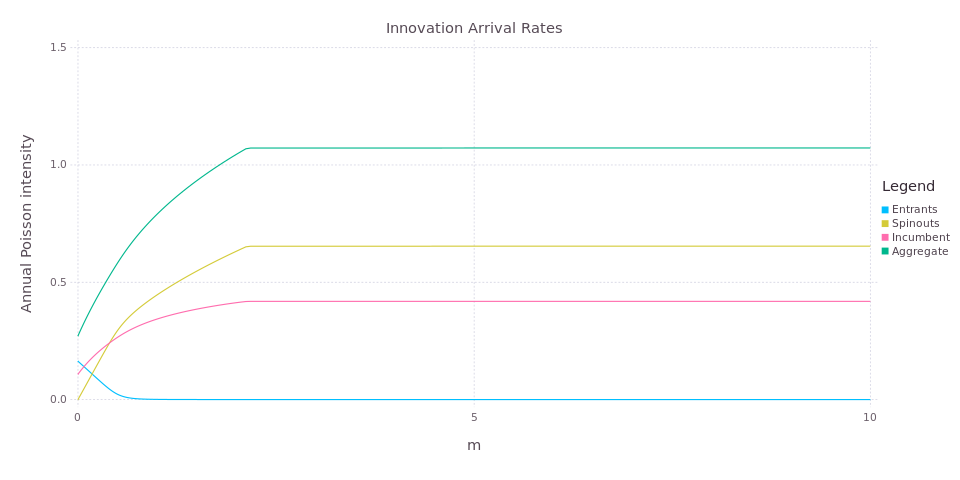
\includegraphics[scale=0.5]{../code/julia/figures/presentation/innovation_rates.png}
	\caption{Above shows the equilibrium innovation (annual) hazard rates over the evolution of a product. The hazard rate of innovation increases as (1) more spinouts enter and (2) incumbents do more R\&D to escape the competition they have created.}
	\label{innovation_rates}
\end{figure}

\subsection{Comparative statics}

Figure \ref{nuxi_chiS_gCompStat} shows the growth implications of varying the rate of employee learning. Equilibrium growth is inverse-U shaped in $\nu \xi$, with a peak shifting to the right as $\chi_S$ is increased. This reflects the tradeoffs discussed in the theory section.

\begin{figure}[h] \phantomsection
 	\centering
	\includegraphics[scale=0.5]{../code/julia/figures/presentation/nuxi_chiS_g_plot_2.png}
	\caption{Implications of $\nu \xi$ and $\chi_S$ for the growth rate $g$ and the R\&D labor allocaiton $L_{RD}$. Both effects are non-monotonic, with peaks that are increasing in $\chi_S$.}
	\label{nuxi_chiS_gCompStat}
\end{figure}

Figure \ref{nuxi_growthDecomposition} shows the decomposition of growth and R\&D employment by incumbents, spinouts and entrants as $\nu \xi$ varies, holding $\chi_S$ constant at the calibrated value. The contribution of spinouts to growth increases as $\nu \xi$ increases, while the contribution of ordinary entrants to growth decreases. These largely offset each other. The contribution of incumbents to growth increases at first and then decreases gradually as $\nu \xi$ increases. 

The top panel of Figure \ref{nuxi_growthDecomposition} shows the R\&D employment. Incumbent firms employ less than 1/10 of the R\&D workers as potential entrants (including spinouts), but lead end up with 1/4 of the growth contribution. This is due to the assumptions on the relative R\&D productivity of entrants and incumbents. As this appears to be at odds with the data, this warrants further investigation.

\begin{figure}[h] \phantomsection
	\centering
	\includegraphics[scale=0.5]{../code/julia/figures/presentation/nuxi_RDandGrowth_plot.png}
	\caption{Growth and R\&D spending decompositions. The bottom panel shows the equilibrium growth decomposition as a function of $\nu \xi$. As $\nu \xi$ increases, the incumbent contribution to growth (blue) increases, but eventually it begins to decrease. Non-spinout entrant contribution to growth decreases monotonically as $\nu \xi$ increases, and the reverse is true for the spinout contribution. The top panel shows R\&D labor used by incumbents, entrants and spinouts. The calibration that incumbents are more productive at R\&D than entrants or spinouts means that incumbents can contribute half as much to growth as entrants / spinouts while deploying 10\% of the R\&D labor. This seems at odds with the data, suggesting I may need to modify my model to account for this.}
	\label{nuxi_growthDecomposition}
\end{figure}

Figure \ref{nuxi_chiS_welfare} shows the welfare effects of varying $\nu \xi$ and $\chi_S$. As in the previous comparative statics, welfare is non-monotonic in $\nu \xi$ given $\chi_S$, with a peak that is increasing in $\chi_S$. As noted previously, increasing $\nu \xi$ expands the production possbilities frontier of the economy. Hence, the decrease in welfare is a lower bound on the inefficiency of the model. In the current calibration, peak decentralized welfare is at $\nu \xi \approx 0.4$. Of course, since I have not solved the planner's problem, the equilibrium may very well still be inefficient at this value. 

Finally, inspecting Figure \ref{nuxi_chiS_welfare} shows that the model predicts substantial welfare gains from increasing the calibrated value of $\nu \xi = 0.1$ to $\nu \xi = 0.4$, of approximately 5\%. This may not be a policy instrument available to the policy maker or even social planner, but it suggests that in this range, relaxing restrictions on spinout formation could significantly improve welfare. 

\begin{figure}[h] \phantomsection
	\centering
	\includegraphics[scale=0.5]{../code/julia/figures/presentation/nuxi_chiS_welfare_plot.png}
	\caption{Welfare implications of varying $\nu \xi$ and $\chi_S$. Welfare is non-monotonic in $\nu \xi$, even though this expands the production possibilities frontier. Peak decentralized welfare is increasing in $\chi_S$.}
	\label{nuxi_chiS_welfare}
\end{figure}


\section{Conclusion}\label{conclusion}

(in progress)

%\nocite{*}
\bibliography{references.bib}








\end{document}